\section{Architectural design}
\label{sect:overalldescription}

\subsection{Overview: High-level components and their interaction}
\label{subsect:Overview:Highlevelcomponentsandtheirinteraction}
\begin{figure}[h!]
    \centering
    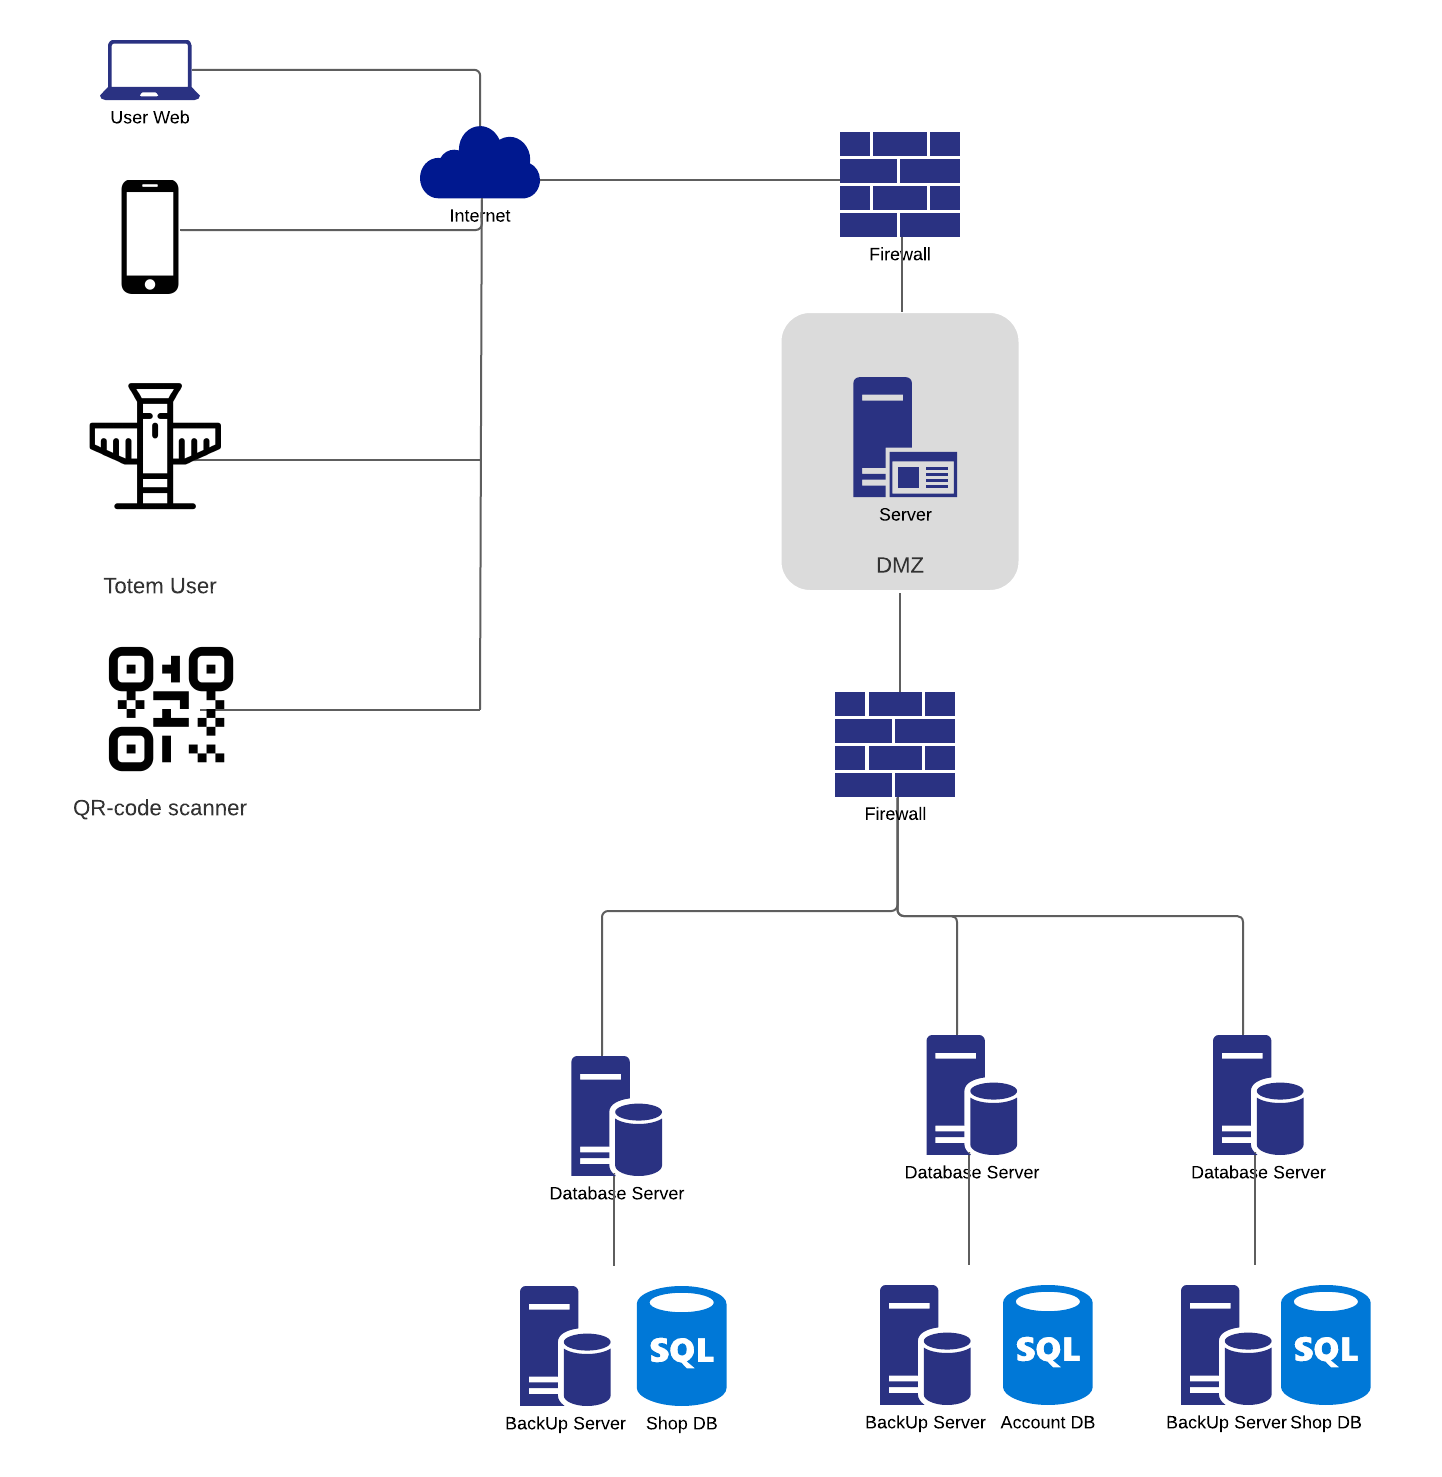
\includegraphics[width=0.6\textwidth]{Images/PhysicalDiagram.png}
    \caption{\label{fig:PhysicalDiagram}{Physical Diagram}}
\end{figure}
The architecture of the system can be summed up in three logical layer: presentation layer, application layer and data layer.
In the image we can see that there are four kind of harware hosting the front-end side of the application: Mobile Users, Totem Users, Laptop Users and the scanner of QR-codes. The latter won't host software implemented by us, but provided by third parties, so it won't be discussed in the rest of the document, exception made for the management of its outgoing http requestes. For all of the other users, the hosted software will be implemented by us and discussed later on in the document.
In any case, the presentation layer will be in part on the client tier and in part of the web tier. 
All of the clients will have access to the application layer through the Web Server, via HTTPS protocol, which is hosting a Gateway Load Balancer in order to efficiently dispatch the incoming requestes towards the correct services. Each service is hosted on a dedicated server, in order to maximize decoupling and scalability. 
Similiarly, it will be implemented a dedicated DataBase Server for each service, which, periodically, will store critical data in a decicated BackUp Server.

\subsection{Component view}
\label{subsect:componentview}
The following diagrams show the main components of the system and the interfaces through which they interact:
\begin{itemize}
    \item The client side is made of four components, which refer to the qr-code scanner application, to the web users and to the mobile application users.
    \item The server side is divided in three subsystems, each of them implements a specific service of the application. For the sake of clarity three different diagram has been modelled. The subsystems are:
    \begin{itemize}
        \item Queue Services Subsystem: it provides the interfaces needed either by managers and users in order to accesses to the functions correlated to the tickets, either queue tickets or visit tickets.
        \item Shop Services Subsystem: it provides the interfaces needed by managers and users in order to accesses to the functions correlated to the shop.
        \item Account Manager Services: it provides the interfaces needed to manage the accounts and also implements some security feature.
    \end{itemize}
\end{itemize}
\begin{figure}[h!]
    \centering
    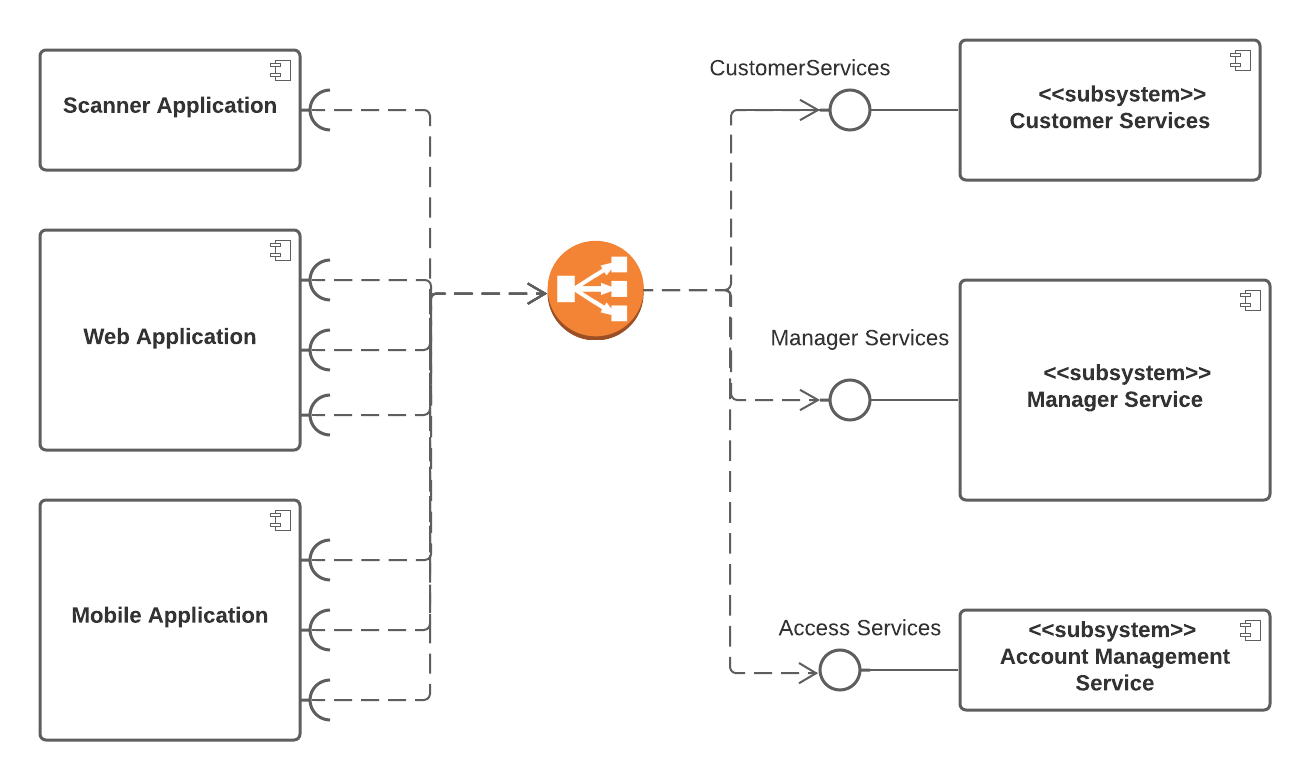
\includegraphics[width=0.6\textwidth]{Images/ComponentViewHighLevel.png}
    \caption{\label{fig:ComponentViewHighLevel}{General component view}}
\end{figure}

\textbf{Queue Service Subsystem Projection}
This service is divided into four modules: \textit{Service Registration Module, Queue Customer Module, Queue Information Module, Queue Manager Module}. 
The \textit{Service Registration Module} is a module dedicated to the registration of the runtime instances to this service.
The \textit{Queue Customer Module} is a module dedicated to functions exploited by the user. Indeed, it is futher splitted into two submodules: \textit{Book Visit Submodule} and \textit{Enqueuement Module}. 
Intuitivily, the first one will implement an interface thanks to which the user will be able to book a visit, to cancel a previously booked visit and to retrieve information about their booked visits.
On the other hand, the second one will implement an interface thanks to which the user will be able to enqueue and dequeue.
The \textit{Queue Information Module} is a module dedicated to function exploited by users and managers, since it allows a client to retrieve information about the virtual queue of a shop.
The \textit{Queue Manager Module} is a module dedicated to function exploited by managers, it offers the possibility to cancels visits in case of emergency.
In order to implement all of these functions, this component needs to have access to its dedicated database.

\begin{figure}[h!]
    \centering
    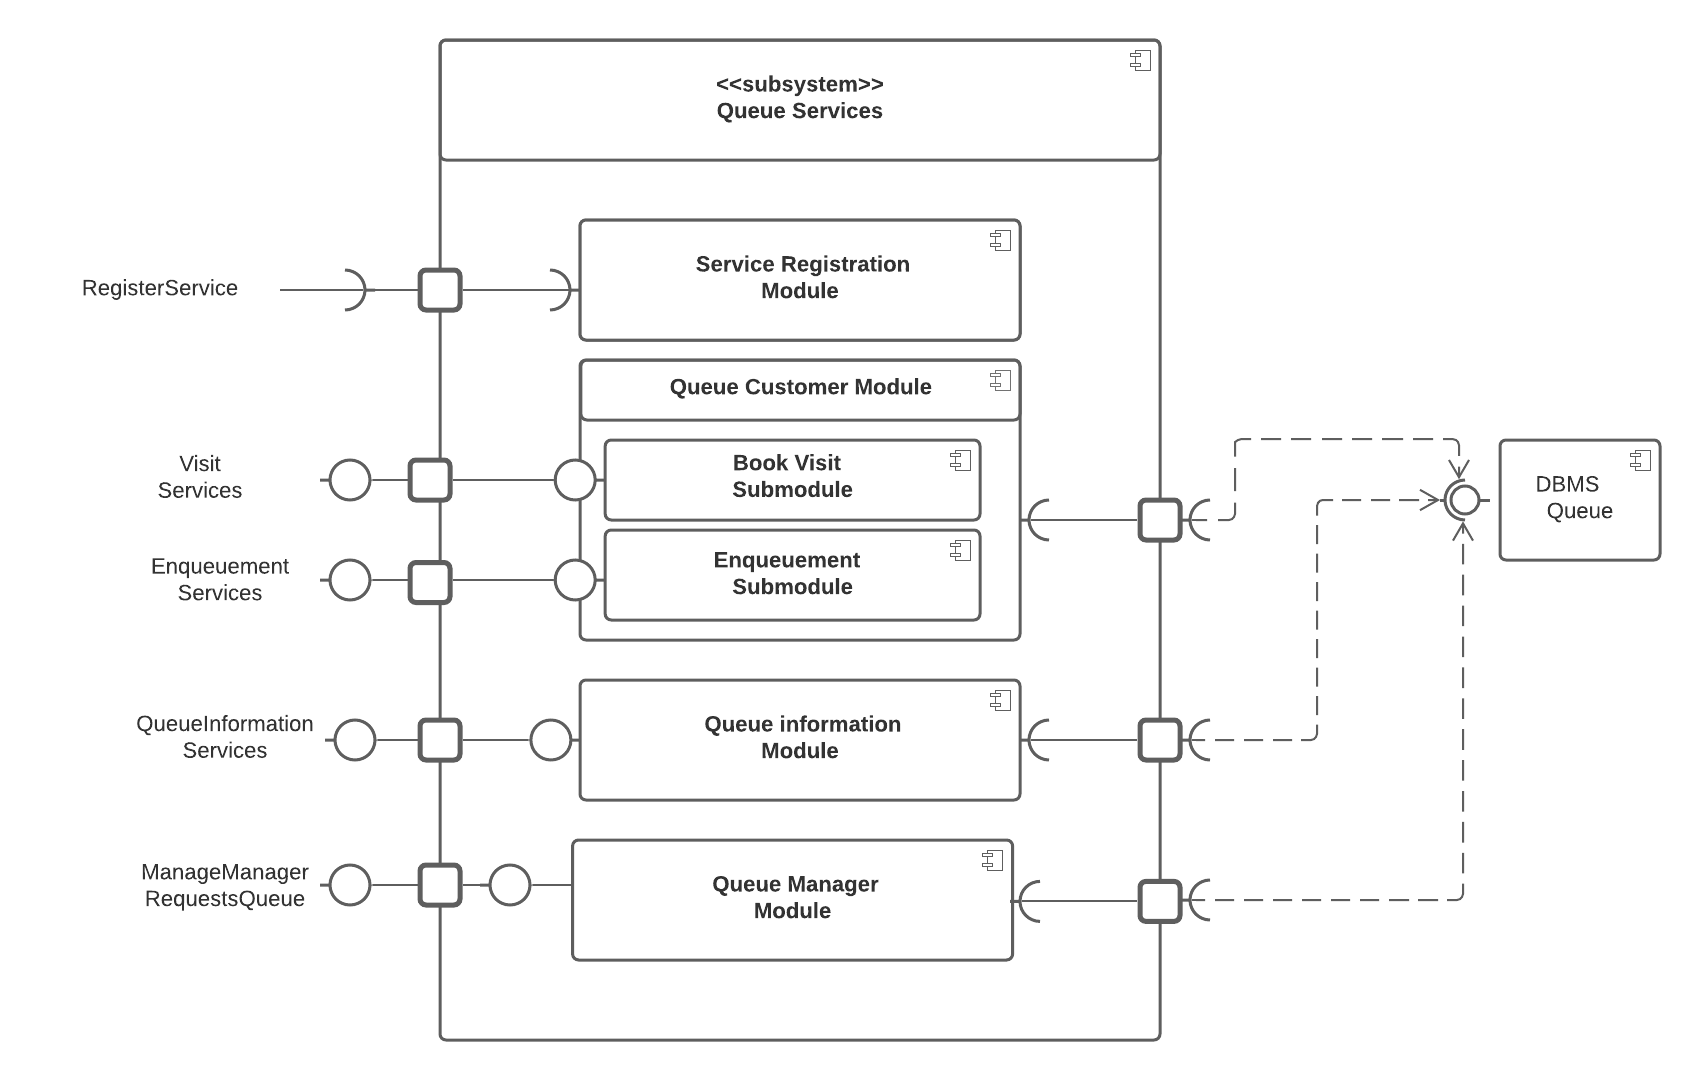
\includegraphics[width=0.6\textwidth]{Images/ComponentViewQueueService.png}
    \caption{\label{fig:ComponentViewQueueServices}{General component view}}
\end{figure}


\textbf{Shop Service Subsystem Projection}
This service is divided into three modules: \textit{Service Registration Module, Manage Shop Module, Shop information Module}. 
The \textit{Service Registration Module} is a module dedicated to the registration of the runtime instances to this service.
The \textit{Manage Shop Module} is a module dedicated to function exploited by the managers. It implement an interface which will allow a manager to add a shop and to update the information of a shop already registered in the system.
The \textit{Shop Information Module} is a module dedicated to function exploited by the managers and the users. It implement an interface which will provide functions to retrieve information about a shop.
In order to implement all of these functions, this component needs to have access to its dedicated database. It also needs to communicate to the Maps Api.

\begin{figure}[h!]
    \centering
    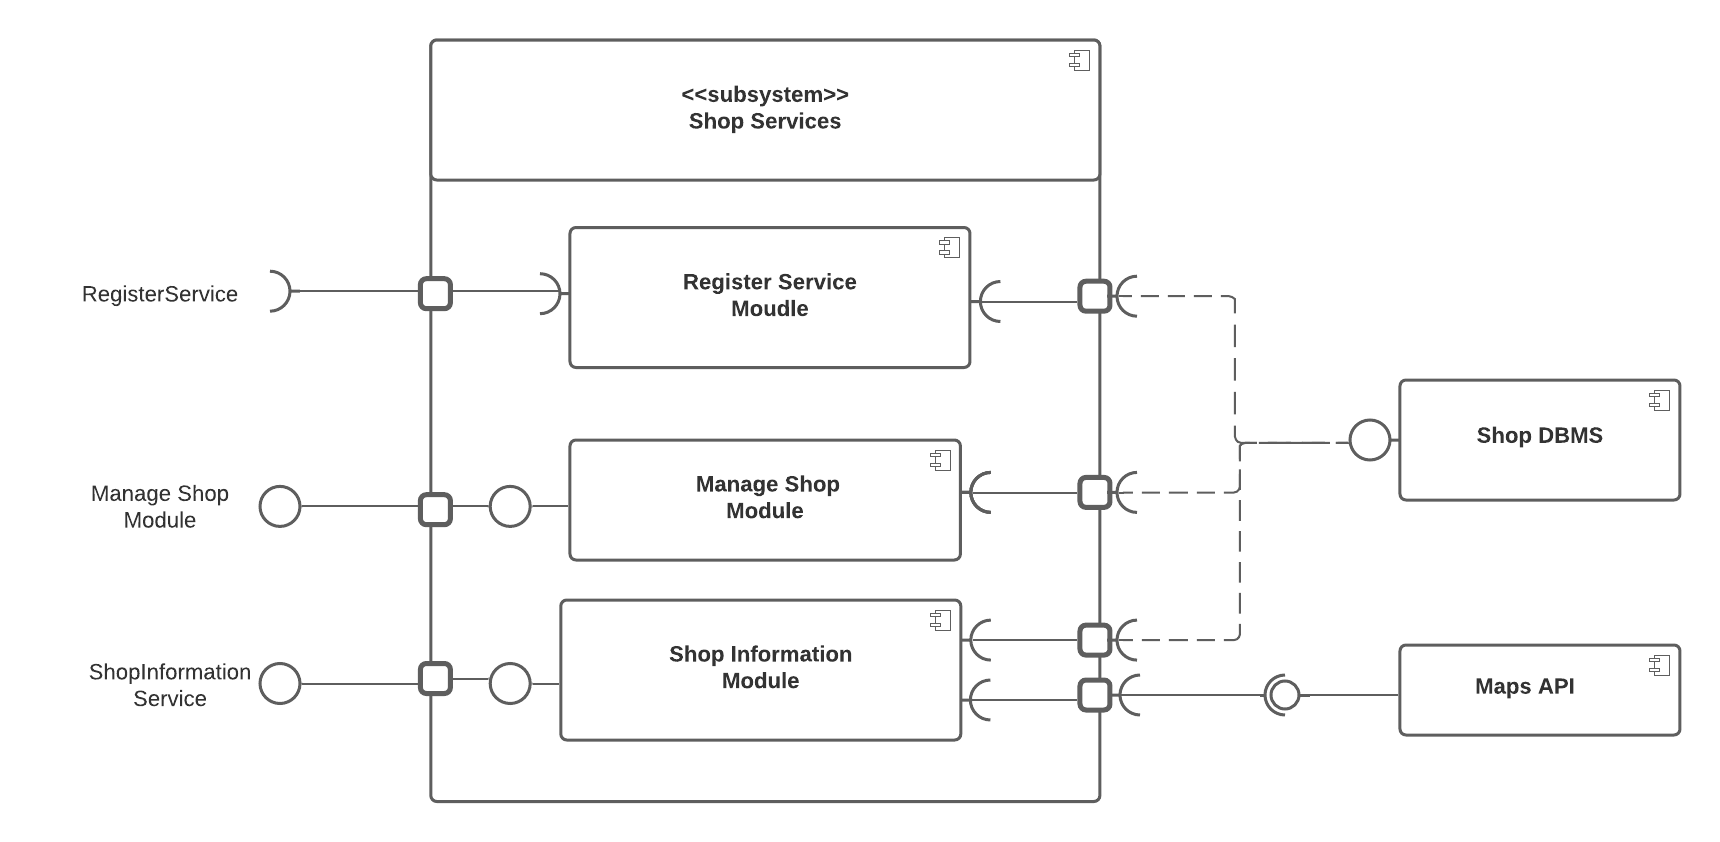
\includegraphics[width=0.6\textwidth]{Images/ComponentViewShopServices.png}
    \caption{\label{fig:ComponentViewShopServices}{General component view}}
\end{figure}

\textbf{Account Manager Subsystem Projection}
This service is divided into two modules: \textit{Service Registration Module, Account Management Module}. 
The \textit{Service Registration Module} is a module dedicated to the registration of the runtime instances to this service.
The \textit{Account Management Module} provides an interface with the functions needed in order for a user or a manager to log in and sign up in the application. It will implement authentication and authorization. 
In order to implement all of these functions, this component needs to have access to its dedicated database. It needs to communicate with a SMSGateway in order to provide some of the functions of authentication. 

\begin{figure}[h!]
    \centering
    \caption{\label{fig:ComponentViewAccountManagerServices}{General component view}}
\end{figure}




\subsection{Entity-relationship diagram}
\label{subsect:entityrelationshipdiagram}

TODO:FEDE

\subsection{Deployment view}
\label{subsect:deploymentview}
The system architecture is a 4-Tier architecture, it is based on the JEE framework and it's typical of a Service Oriented Application:
\begin{itemize}
    \item \textbf{TIER 1} is the client tier, it is composed by the mobile applications, the totems and the users browsers and the qr-code scanner application. All of them will communicate with the web server via the HTTPS protocol.
    \item \textbf{TIER 2} is composed by the web server, implemented with Apache Tomcat. It is composed by the static content module and by and ELB, used as gateway and to implement additional security features.
    \item \textbf{TIER 3} it's the Application Tier. Three server will hosts three different artifact, one for each service. The OS chosen is CentOs and the execution enviroment TomEE.
    \item \textbf{TIER 4} is the Data Tier. The connection beetween Tier 3 and 4 is performed via JDBC connector which uses jdbc protocol.
\end{itemize}
\begin{figure}[h!]
    \centering
    \includegraphics[width=0.6\textwidth]{Images/Deployement View.png}
    \caption{\label{fig:Deployement View}{General component view}}
\end{figure}

copiata micidiale da power enjoy

\subsection{Runtime view}
\label{subsect:runtimeview}

user search a shop

user book a visit/user enqueue (sono molto simili..)

customer line up (totem)

QR-code scanner

Manager cancels a customer visit

\subsection{Component interfaces}
\label{subsect:componentinterfaces}

Facciamo interfacce come power enjoy e specifichiamo che a ogni metodo corrisponde una servlet, e che il mezzo di comunicazione è HTTP, quindi non avremo effettivamente queste interfacce

\subsection{Selected architectural styles and patterns}
\label{subsect:selectedarchitecturalstylesandpatterns}

MVC

OBSERVER (per la view di sicuro, per il resto boh, dobbiamo capirlo)

CHAIN OF RESPONSIBILITY PATTERN – In this design pattern a request from a client can be handled by a number of handler or receiver objects. So basically, the client request is passed down each handler in the chain until a handler that can process the request is found. Servlet filters are a classic example of the Chain of Responsibility pattern. Spring has a class called HandlerInterceptorAdapter which is also an example of the Chain of Responsibility pattern. It has a method called preHandle, which follows the chain of responsibility pattern. Both servlet filters as well as Spring interceptors can be used to house code that is common for all requests like logging or authentication and that is separate from the business logic.

FACADE

SIGLETON - maybe

STRATEGY - maybe

POOL PATTERN - connection pooling patern JDBC - oppure no se usiamo JPA

TOMCAT GESTISCE LO SCHEDULING DEGLI EVENTI TEMPORALI..

\subsection{Other design decisions}
\label{subsect:otherdesigndecisions}


